%----------------------------------------------------------------------------------------
%	PACKAGES AND OTHER DOCUMENT CONFIGURATIONS
%----------------------------------------------------------------------------------------
\documentclass[twoside]{article}

\usepackage[sc]{mathpazo} % Use the Palatino font
\usepackage[english]{babel}
\usepackage[utf8]{inputenc}
\usepackage{lipsum}
\usepackage{graphicx}
%\usepackage[T1]{fontenc} % Use 8-bit encoding that has 256 glyphs
\linespread{1.15} % Line spacing - Palatino needs more space between lines
\usepackage{microtype} % Slightly tweak font spacing for aesthetics

\usepackage[hmarginratio=1:1,top=32mm,columnsep=20pt]{geometry} % Document margins
\usepackage{multicol} % Used for the two-column layout of the document
\usepackage[hang, small,labelfont=bf,up,textfont=it,up]{caption} % Custom captions under/above floats in tables or figures
\usepackage{mathtools}
\usepackage{booktabs} % Horizontal rules in tables
\usepackage{float} % Required for tables and figures in the multi-column environment - they need to be placed in specific locations with the [H] (e.g. \begin{table}[H])
\usepackage{hyperref} % For hyperlinks in the PDF
\usepackage{wrapfig}
%\usepackage[]{mcode} % For embebing matlab code
\usepackage[makeroom]{cancel}

%\usepackage{lettrine} % The lettrine is the first enlarged letter at the beginning of the text
\usepackage{paralist} % Used for the compactitem environment which makes bullet points with less space between them

\usepackage{abstract} % Allows abstract customization
\renewcommand{\abstractnamefont}{\normalfont\bfseries} % Set the "Abstract" text to bold
\renewcommand{\abstracttextfont}{\normalfont\small\itshape} % Set the abstract itself to small italic text
\newcommand{\cl}{clearly blue }

\usepackage{titlesec} % Allows customization of titles
%\renewcommand\thesection{\Roman{section}} % Roman numerals for the sections
%\renewcommand\thesubsection{\Roman{subsection}} % Roman numerals for subsections
\titleformat{\section}[block]{\large\scshape\centering}{\thesection.}{1em}{} % Change the look of the section titles
\titleformat{\subsection}[block]{\large\centering}{\thesubsection.}{1em}{} % Change the look of the section titles

\usepackage{fancyhdr} % Headers and footers
\pagestyle{fancy} % All pages have headers and footers
\fancyhead{} % Blank out the default header
\fancyfoot{} % Blank out the default footer
\fancyhead[C]{Experimental Optics % based on TRACS 
\hspace{4pt} $\bullet$ \hspace{4pt} Diffraction Gratings
\hspace{4pt} $\bullet$ \hspace{4pt} Marzo 2018} % Custom header text
\fancyfoot[RO,LE]{\thepage} % Custom footer text

\usepackage{cite}

\DeclareGraphicsExtensions{.pdf,.png,.jpg} % Graphics type

%----------------------------------------------------------------------------------------
%	   TITLE SECTION
%----------------------------------------------------------------------------------------

\title{
	\vspace{-15mm}
	\fontsize{28pt}{10pt}
	\selectfont\textbf{Characterizing Diffraction Gratings}%Characterizing Diffraction Gratings: Measurement of an atomic transition wavelength}% Article title
}

\author{
	\large
	\textsc{Jaime Díez González-Pardo}\\[4mm]%\thanks{A thank you or further information}\\[2mm] % Your name
	\fontsize{28pt}{10pt} University of Cantabria \\ % Your institution
	%\thanks{A thank you or further information}\\[2mm] % Your name
	\normalsize Experimental Optics \\ 
	%\normalsize{Compañera:} \textsc{Mónica Escobedo}\\%\normalsize \href{mailto:john@smith.com}{john@smith.com} % Your email address
	%\vspace{5mm}
}

\date{ \today }


%----------------------------------------------------------------------------------------
%      · DOCUMENT
%----------------------------------------------------------------------------------------

\begin{document}


	\maketitle % Insert title


	\thispagestyle{fancy} % All pages have headers and footers

%----------------------------------------------------------------------------------------
%	  ABSTRACT
%----------------------------------------------------------------------------------------

	\begin{abstract}

		\noindent% Dummy abstract text

		It has been studied the diffraction phenomenon produced by a grating for the ligth emited from a Cd atomic lamp, obtainig its spectral lines. First of all it has been necessary to obtain the grating parameter with a value of $\bar{d} = (884.4 \pm 0.8) \textrm{ nm}$, from the diffraction angle $\theta$ of a well-known spectral line, in order to characterize the diffraction grating. In this way it has been able to obtain the wavelength of another unknown wavelength, with a result $\bar{\lambda} = (508.6 \pm 0.5) \textrm{ nm}$ compatible with the real wavelength for that line. 

	\end{abstract}

%----------------------------------------------------------------------------------------
%	  ARTICLE CONTENTS
%----------------------------------------------------------------------------------------

	\begin{multicols}{2} % Two-column layout throughout the main article text

		\section{Introduction} % Scope of the project = rad effects + minimization

			Gratings can produce diffraction on an incident ligth, as long as its wavelength and distances between slots (the grating parameter $d$) are in the same order of magnitud, due to interferences between beams which have been passed thru differents slots. If the difference between optics path is a multiple of wavelength, the interference will be constructive, obtaining a maximum. This condition is fulfilled only by some directions for a given grating parameter $d$ as it is shown for a normal incident beam, in the equation \ref{eq:Bragg}, where $\theta$ is the angle formed by the normal to the surface grating and the diffracted direction. 

				\begin{equation}
					2 d \sin \theta = m \lambda
					\label{eq:Bragg}
				\end{equation}

			Following the equation \ref{eq:Bragg}, if either the wavelength $\lambda$ or the grating parameter $d$ is known, the other can be obtain by measure the angle $\theta$.

			Due to the parameter $d$ of the grating used in the experimental set-up is unknown, it is going to try to obtain by measure the angles $\theta$ for the diffraction of a spectral line with well-known wavelength. Once $d$ is known it is possible to obtain any wavelength of a diffracted line. 


		\section{Method}

			The light source used is a spectral lamp of Cd atomic gas, with well-known wavelength for the clear blue emission line $\lambda = 480.0 nm$ \cite{Chema}.

			All measurements have been made by means of a goniometer with two differents arms. The collimator arm is placed just after the spectral lamp in order to drives the incident beam from the source onto the grating. The second arm contains a telescope attached to a rotating disk with a lateral scale that indicates its angular position with a precision of $1'$ arc. The zero of the scale is in a lateral window of another rotating disk. This other disk contains a platfom, that can be levelled with three screws, in which the grating has been put. 

			The different parts of the experimental set-up are shown in the Figure \ref{Img:GnoSqueme}.

				\begin{figure}[H]
					\centering
					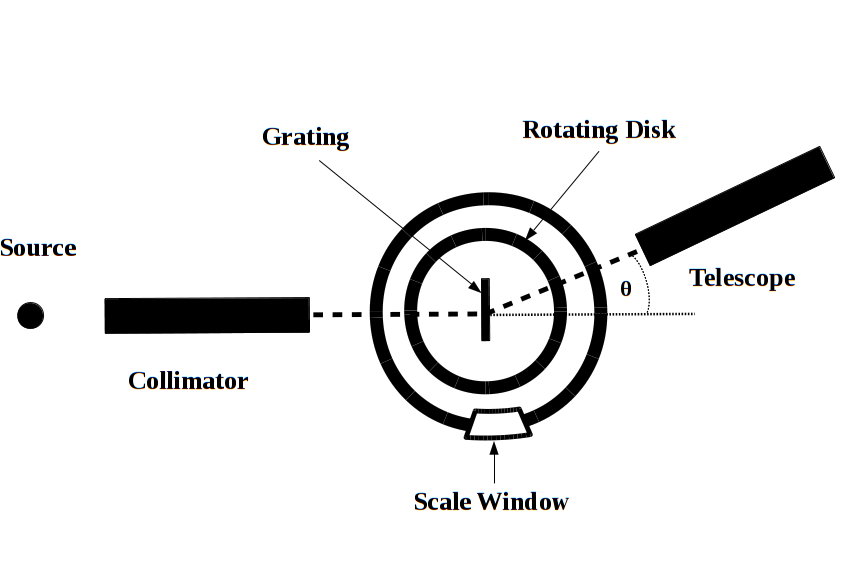
\includegraphics[scale=0.24]{GnoSqueme.png}
					\caption{\label{Img:GnoSqueme}Scheme of the experimental set-up used in the laboratory.}
				\end{figure}

			Before measuring, it is important to check all the set-up, focusing the collimator to see the slit sharp, the telescope to infinity (or a far object), its eyepiece on the cross and setting that cross correctly vertical.

			Another important thing to check is that the grating is as perpendicular as possible to the incident beam. To this purpose it has been measured the position of the telescope where the slit's image is centred $\theta_{middle}$, and then the position of the \cl line of the spectrum diffracted in the first order at the right side $\theta_r$ and at the left side $\theta_l$. If the grating is completely perpendicular to the incident beam, the angle between $\theta_{middle}$ and, both $\theta_r$ and $\theta_l$, should be the same. In the case the difference between both angles is larger than $5'$ arc the platform has to be rotate  slightly by means of the screws, and the measurements repeated.

			Once the experimental set-up is correctly disposed it is able to start characterizing the diffraction grating. First, the diffraction grating parameter will be obtain by measure the positions $\theta_r$ and $\theta_l$ of the \cl line obtaining the diffraction angle $\theta = \frac{\theta_r-\theta_l}{2}$. In order to minimize the error it is going to be taken six measurements of $\theta$. After calculate the average $\bar{\theta}$, $\bar{d}$ will be obtain by the equation \ref{eq:Bragg}.

			In the last part of the experiment it has been tried to obtain the wavelength of another spectral line from the former value of $\bar{d}$ and the new average angle $\bar{\theta}$. The method used to obtain the new $\bar{\theta}$ is the same used for the \cl line but for the new spectral line.
 
		\section{Results}

			Most of the angle values shown in the report are express in therms of degrees using the conversion of the equation \ref{eq:conversion}, although they were taken in degrees and minutes in order to simplify the results and the calculations.

				\begin{equation}
					1' = \left(\frac{1}{60}\right)^o
					\label{eq:conversion}
				\end{equation}

			The first part of the experiment correspond to the alignment of the diffraction grating, which had to be rotated once to achieve a final value for the differences between both angles of $\delta \theta \approx 4'$ arc.

				\begin{equation}
					|\theta_r - \theta_{middle}| - |\theta_l - \theta_{middle}| \approx 4' < 5'
					\label{eq:perpendicular}
				\end{equation}

			In the Table \ref{Tab:Perpendicular} appear all the values of $\theta_{middle}$, $\theta_{r}$, $\theta_{l}$ and $\delta \theta$ obtained before and after adjust the platform of the grating.

				\begin{table}[H]
	\centering
	\begin{tabular}{ c  c  c  c }
		\\\hline
		\centering
			$\theta_{middle}/^o$ & $\theta_{l}/^o$ & $\theta_{r}/^o$ & $\delta\theta$ \\\hline
			91.583 & 75.750 & 107.300 & 7' \\
			91.383 & 75.567 & 107.133 & 4' \\\hline
	\end{tabular}
	\caption{\label{Tab:Perpendicular}Positions of the telescope for the slit's image $\theta_{middle}$, the first order diffracted \cl line at the left side $\theta_{l}$, at the right side $\theta_{r}$, and the difference between angles, $\delta \theta$ obtained by the equation \ref{eq:perpendicular}. The error of the positions is $\Delta \theta = 0.017 ^o$.}
\end{table}
 %should have a lavel {Tab:Perpendicular}

			\subsection{Grating Parameter  \texorpdfstring{$d$}{TEXT}}
				\label{sec:dPara}

				In order to obtain the diffraction grating parameter $d$ it has been taken six measurements of the positions $\theta_r$ and $\theta_l$ of the \cl line obtaining the diffraction angle by $\theta = \frac{\theta_r-\theta_l}{2}$. This values appear in the Table \ref{Tab:dParameter}.

					\begin{table}[H]
	\centering
	\begin{tabular}{ c  c  c }
		\\\hline
		\centering
			$\theta_{l}/^o$ & $\theta_{r}/^o$ & $\theta/^o$ \\\hline
			75.567 & 107.133 & 15.783 \\
			75.667 & 107.067 & 15.700 \\
			75.583 & 107.100 & 15.758 \\
			75.617 & 107.050 & 15.717 \\
			75.550 & 107.117 & 15.783 \\
			75.617 & 107.083 & 15.733 \\\hline
	\end{tabular}
	\caption{\label{Tab:dParameter}Positions $\theta_r$ and $\theta_l$ of the \cl line and the diffraction angle $\theta = \frac{\theta_r-\theta_l}{2}$. The error of $\theta_l$ and $\theta_r$ is $\Delta \theta_{l,r} = 0.017^o$. The error of $\theta$ calculated by the equation \ref{eq:err:angles} on the appendix \ref{appendix} is $\Delta \theta = 0.012$.}
\end{table}


				With those values the average angle $\bar{\theta}$ is calculated obtaining a value:

					\begin{equation}
						\bar{\theta} = \frac{1}{N} \sum^{N}_{i=1} \theta_i = (15.746 \pm 0.014) ^o
					\end{equation}

				The error of $\bar{\theta}$ correspond to the standard deviation calculated in the appendix \ref{app:dParameter} by the equation \ref{eq:var:TtaMed}.

				Once $\bar{\theta}$ is calculated, obtain the diffraction parameter is just substitute the known values in the equation \ref{eq:Bragg}.

					\begin{equation}
						\bar{d} = \frac{m \lambda} {2 \cdot \sin(\bar{\theta})} = (884.4 \pm 0.8) \textrm{ nm}
						\label{eq:dMed}
					\end{equation}

				Where $m=1$ accordingly to first order diffraction lines, and $\lambda = 480.0$ nm \cite{Chema}. The error of $\bar{d}$ is calculated in the appendix \ref{app:dParameter} in the equation \ref{eq:var:dMed}

 			\subsection{Unknown Wavelength}
				\label{sec:unKnownWL} 				

 				The same method as the used for the diffraction grating parameter has been used to obtain the wavelength for another spectral line, the green one for this experiment. The Table \ref{Tab:unKnownWL} shown the measurements for the positions.

 					\begin{table}[H]
	\centering
	\begin{tabular}{ c  c  c }
		\\\hline
		\centering
			$\theta_{l}/^o$ & $\theta_{r}/^o$ & $\theta/^o$ \\\hline
			74.667 & 108.067 & 16.700 \\
			74.667 & 108.083 & 16.708 \\
			74.683 & 108.100 & 16.708 \\
			74.700 & 108.100 & 16.700 \\
			74.633 & 108.083 & 16.725 \\
			74.600 & 108.050 & 16.725 \\\hline
	\end{tabular}
	\caption{\label{Tab:unKnownWL}Positions $\theta_r$ and $\theta_l$ of the \cl line and the diffraction angle $\theta = \frac{\theta_r-\theta_l}{2}$. The error of $\theta_l$ and $\theta_r$ is $\Delta \theta_{l,r} = 0.017^o$. The error of $\theta$ calculated by the equation \ref{eq:err:angles} on the appendix \ref{appendix} is $\Delta \theta = 0.012^o$.}
\end{table}


 				As in the former method, the average angle $\bar{\theta}$ is calculated obtaining a value:

					\begin{equation}
						\bar{\theta} = \frac{1}{N} \sum^{N}_{i=1} \theta_i = (16.711 \pm 0.005) ^o
					\end{equation}

				The error of $\bar{\theta}$ correspond to the standard deviation calculated in the appendix \ref{app:unKnownWL} by the equation \ref{eq:var:TtaMed:WL}.

				Once the $\bar{\theta}$ is calculated, obtain the the diffraction parameter is just substitute the known values in the equation \ref{eq:Bragg}.

					\begin{equation}
						\bar{\lambda} = 2 \bar{d} \sin(\bar{\theta}) = (508.6 \pm 0.5) \textrm{ nm}
						\label{eq:WLed}
					\end{equation}

				Where $m=1$ and $\bar{d}$ is the value obtained in the section \ref{sec:dPara}. The error of $\bar{\lambda}$ is calculated in the appendix \ref{app:unKnownWL} in the equation \ref{eq:var:WLMed}

		\section{Discussion}

			A diffraction grating has been characterizing by measured its grating parameter $d$ from the angle $\bar{\theta}$, formed by the normal to the surface grating and the diffracted direction of the spectral \cl line, obtaining a value for it of $\bar{d} = (884.4 \pm 0.8)$ nm. In order to try to minimized the error it has been taken six measurements for the angle $\theta$ using the average to obtain $d$. By this way, a relative error of about $ 0.09 \%$ has been obtained. This error means a very precise value for $d$, which does not necessary implate that the value is correct, due to the manufacture grating parameter value is unknown.

			Once the diffraction grating parameter $d$ has been obtained, it has been tried to calculate the wavelength of the green spectral line of the Cd atomic gas. The wavelength's value obtained is $\bar{\lambda} = (508.6 \pm 0.5) $ nm. It has been used the average angle of six differents measurements of $\theta$ such as in the former method. The relative error obtained is about $1\%$. This error is little bigger than the error obtained for $d$, due to it depends on it and on the standard deviation of $\bar{\theta}$, but again very small, showing that the method used in the experiment provide very precise values. 

			The experimental wavelength obtained is compatible with the known value of the green spectral line for the Cd I ($508.58217$ nm) \cite{NIST_ASD}. With a result as good as the obtained for the $\bar{\lambda}$ and due to it has been obtained from the experimental value of $\bar{d}$, it could be said that the manufacture value of $d$ should be near the experimental one, $\bar{d}$.

			Knowing the diffraction grating parameter it is possible to obtain the wavelength of any spectral line by measurements of the diffracted angle $\theta$, as it has been done for the green spectral line of the Cd. This method could be used in order to determine the spectrum of a certain emitting gas by characterized its spectral lines, been able to identify the gas. 

			However, the diffraction grating used in this experiment could only be used to identify gases with its spectrum in the visible range. This is due to the diffraction phenomenon only occures when the grating parameter and the wavelength of the incident beam have the same order of magnitude.

			A similar method could be used using a glass prism instead the diffraction grating. In this case the prism will dispers the light, been able to observe (and measure) the spectral lines clearly separated. The dispersion produce by the prism is not based in the diffraction phenomenon as in the grating, but the index of refraction of the glass depends on the wavelength, so the ligth will be transmitted from one medium to the other with differents angles depends on the wavelength, separating the spectral lines. 

		\section{Conclussions}

			It has been verify the expression \ref{eq:Bragg} for the diffraction produced by a grating, obtaining the grating parameter $\bar{d}$ and an unknown wavelength $\bar{\lambda}$. It can be said that this experimental set-up could be used to identify a certain gas by characterizing its spectral lines as long as that gas emits in the visible range.

	\end{multicols}
%----------------------------------------------------------------------------------------
%     BIBLIOGRAPHY
%----------------------------------------------------------------------------------------

	\bibliographystyle{unsrt}
	\bibliography{../../biblio}

%----------------------------------------------------------------------------------------
%     APPENDIX
%----------------------------------------------------------------------------------------

%\newpage

	\appendix

		\section{Error Propagation}
			\label{appendix}

			In the sections \ref{sec:dPara} and \ref{sec:unKnownWL} the angles $\theta$ have been obtained from the positions $\theta_r$ and $\theta_l$ by $\theta = \frac{\theta_r - \theta_l} {2}$. The error of those values is calculated by the equation \ref{eq:err:angles} and depends only on the error of $\theta_r$ and $\theta_l$ which are the error given by the instrument ($\pm 0.017 ^o$).

				\begin{equation}
					\Delta \theta = \sqrt{\left(\frac{\Delta\theta_r}{2}\right)^2 + \left(\frac{\Delta\theta_l}{2}\right)^2} = \frac{0.017} {\sqrt{2}} = 0.012^o
					\label{eq:err:angles}
				\end{equation}

			\subsection{Grating Parameter  \texorpdfstring{$d$}{TEXT}}
				\label{app:dParameter}

				In the section \ref{sec:dPara} it has been calculated the average angle $\bar{\theta}$. Its error correspond to the standard deviation calculated in the equation \ref{eq:var:TtaMed}.

					\begin{equation}
						\begin{matrix}

							\sigma^2_{\bar{\theta}} = \frac{1}{N(N-1)} \sum^N_{i=1} (\theta_i - \bar{\theta})^2 & \rightarrow & \sigma_{\bar{\theta}} = \sqrt{\frac{1}{N(N-1)} \sum^N_{i=1}(\theta_i - \bar{\theta})^2} = 0.014^o
						\end{matrix}
						\label{eq:var:TtaMed}
					\end{equation} 

				The error of the $\bar{d}$ calculated in the equation \ref{eq:dMed} is obtained by the following equation \ref{eq:var:dMed}.

					\begin{equation}
						\sigma_{\bar{d}} = \sqrt{ \left[ \frac{\lambda \cos(\bar{\theta})}{2\sin^2(\bar{\theta})} \right]^2 \sigma^2_{\bar{\theta}}} = 0.78 nm
						\label{eq:var:dMed}
					\end{equation}
	 
			\subsection{Unknow Wavelength}
				\label{app:unKnownWL}

				In the section \ref{sec:unKnownWL} it has been calculated the average angle $\bar{\theta}$. Its error correspond to the standard deviation calculated in the equation \ref{eq:var:TtaMed}.

					\begin{equation}
						\begin{matrix}

							\sigma^2_{\bar{\theta}} = \frac{1}{N(N-1)} \sum^N_{i=1} (\theta_i - \bar{\theta})^2 & \rightarrow & \sigma_{\bar{\theta}} = \sqrt{\frac{1}{N(N-1)} \sum^N_{i=1}(\theta_i - \bar{\theta})^2} = 0.005^o
						\end{matrix}
						\label{eq:var:TtaMed:WL}
					\end{equation} 

				The error of the $\bar{d}$ calculated in the equation \ref{eq:WLed} is obtained by the following equation \ref{eq:var:WLMed}.

					\begin{equation}
						\sigma_{\bar{\lambda}} = \sqrt{ (2\sin(\bar{\theta}))^2 \sigma_{\bar{d}}^2 + (2 \bar{d} \cos(\bar{\theta}))^2 \sigma^2_{\bar{\theta}}} = 0.47 nm
						\label{eq:var:WLMed}
					\end{equation}


\end{document}

%--------------------------------------------------------------------------------------
%            TEMPLATES
%--------------------------------------------------------------------------------------

%----------------------------------------------------------------------------------------
%            how to insert an image
%----------------------------------------------------------------------------------------

%	\begin{figure}[H]
%		\centering
%		\includegraphics[scale= ]{nombre de la imagen.jpg}
%		\caption{\label{Img:widgets}el pie de pagina que le quieras 	poner a la imagen}
%	\end{figure}
 
%----------------------------------------------------------------------------------------
%            how to insert a table
%----------------------------------------------------------------------------------------

%	\begin{table}[H]
%		\centering
%		\begin{tabular}{|c|c|c|c|}
%			\hline
%			\centering
%				Altura(h) & Distancia (d) & Elaboracion (e) & Longitud (l) \\
%				($\pm0.5$ mm) & ($\pm0.5$ mm) & ($\pm0.5$ mm) & ($\pm0.5$ mm) \\ \hline
%				 &  &  &  \\ \hline
%				 &  &  &  \\ \hline
%				 &  &  &  \\ \hline
%				 &  &  &  \\ \hline
%				 &  &  &  \\ \hline
%		         &  &  &  \\ \hline
%		\end{tabular}
%		\caption{\label{Tab:widgets}pie de pagina que le quieras poner}
%	\end{table}

%----------------------------------------------------------------------------------------
%             How to remove the label in equactions
%----------------------------------------------------------------------------------------

%	\begin{equation*}
%		
%	\end{equation*}

%----------------------------------------------------------------------------------------
%              How to set bibliography
%----------------------------------------------------------------------------------------

%\bibliographystyle{unsrt}
%\bibliography{biblio}
%
%Then you have to set a .bib document such as the next template
%
%	@book{nickname,
%	author = {},
%	title = {},
%	edition = {},
%	year = {},
%	volume = {},
%	ISBN = {}
%	}
%
%	@ARTICLE{nickname,
%	author = {},
%	title = {},
%	year = {},
%	volume = {},
%	}


%----------------------------------------------------------------------------------------
%              END
%----------------------------------------------------------------------------------------